\documentclass[a4paper,10pt]{article}
\usepackage[brazilian]{babel}
\usepackage[T1]{fontenc}
\usepackage[utf8]{inputenc}
\usepackage{lmodern}
\usepackage{geometry}
\geometry{verbose,tmargin=3cm,bmargin=3cm,lmargin=2cm,rmargin=2cm}
\usepackage{fancyhdr}
\pagestyle{fancy}
\usepackage{amsthm}
\usepackage{amsmath}
%\numberwithin{equation}{section}
\usepackage{amsfonts}
\usepackage{amssymb}
\usepackage{mathtools}
%\usepackage{mnsymbol}
\usepackage[authoryear]{natbib}
\usepackage{algorithm}
\usepackage{algpseudocode}
\usepackage[hyphens]{url}
\usepackage{color}
\usepackage{graphicx}
\usepackage{xcolor}
\usepackage{import}
\usepackage{bm}
\usepackage{cancel}
\usepackage{listings}
\usepackage{graphicx}
\usepackage{caption}
\usepackage{subcaption}
\graphicspath{{Figures/}}

\usepackage{xcolor}

\definecolor{codegreen}{rgb}{0,0.6,0}
\definecolor{codegray}{rgb}{0.5,0.5,0.5}
\definecolor{codepurple}{rgb}{0.58,0,0.82}
\definecolor{backcolour}{rgb}{0.95,0.95,0.92}

\lstdefinestyle{mystyle}{
	backgroundcolor=\color{backcolour},   
	commentstyle=\color{codegreen},
	keywordstyle=\color{magenta},
	numberstyle=\tiny\color{codegray},
	stringstyle=\color{codepurple},
	basicstyle=\ttfamily\footnotesize,
	breakatwhitespace=false,         
	breaklines=true,                 
	captionpos=b,                    
	keepspaces=true,                 
	numbers=left,                    
	numbersep=5pt,                  
	showspaces=false,                
	showstringspaces=false,
	showtabs=false,                  
	tabsize=2
}

\lstset{style=mystyle}

\makeatletter
\usepackage[colorlinks=true,linkcolor=red]{hyperref}
\makeatother




\bibliographystyle{apalike2}

\begin{document}
% ------------------ NOTA -----------------------
%
% 1 - Você não precisa alterar o arquivo de template, somente esse arquivo.
% 2 - Abaixo de cada comando há uma nota que o auxiliará a preencher os campos. Todos os
%     comandos são auto-explicáveis, mas as notas o ajudarão em caso de dúvidas.
%
% -----------------------------------------------

\newcommand{\surname}{RAFFO}
% Substitua "SOBRENOME" por ADORNO, RAFFO ou PIMENTA, conforme quem for o seu orientador.
% No caso de haver um co-orientador, use as três primeiras letras de cada sobrenome separadas
% por '/'. Por exemplo, se seu orientador é o Prof. Adorno e seu co-orientador é o Prof.
% Pimenta, escreva ADO/PIM.

\newcommand{\initials}{JMC}
% Coloque suas iniciais aqui (ex., Bruno Vilhena Adorno = BVA)

\newcommand{\reportnumber}{1}
% Mude "X" pelo número do relatório

\newcommand{\reportversion}{1}
% Mude "Y" pelo número da versão do relatório.

\newcommand{\reporttitle}{\textbf{Parallel Distributed Compensator(PDC) de um Pendulo Invertido Via Representação Takagi-Sugeno}}

\newcommand{\registrationnumber}{2016086496}

\newcommand{\studentname}{Jonatan Mota Campos}

\newcommand{\advisorname}{Guilherme Vianna Raffo}

\newcommand{\coadvisorname}{}

\newcommand{\macroheader}[4]{MACRO/#1--\the\year /#2/#3+Versão-#4}


\lfoot{\noindent \macroheader{\surname}{\initials}{\reportnumber}{\reportversion}}


\cfoot{}


\rhead{\noindent 
\includegraphics[width=0.15\textwidth]{report_template/macro_inline}}


\rfoot{\thepage}


\lhead{\leftmark}

\thispagestyle{empty}

\noindent \begin{center}
\textbf{}%
\begin{minipage}[t]{1\columnwidth}%
\noindent \begin{center}
\textbf{}%
\begin{minipage}[c]{0.3\columnwidth}%
\noindent \begin{flushleft}

\includegraphics[width=1\textwidth]{report_template/macro_inline_name}
\par\end{flushleft}%
\end{minipage}\textbf{}%
\begin{minipage}[b]{0.7\textwidth}%
\noindent \begin{flushright}
\textbf{\macroheader{\surname}{\initials}{\reportnumber}{\reportversion}}
\par\end{flushright}%
\end{minipage}
\par\end{center}%
\end{minipage}
\par\end{center}

\noindent \rule[0.5ex]{1\textwidth}{1pt}

\bigskip{}


\begin{center}
\textbf{\Large{}Universidade Federal de Minas Gerais - UFMG}
\par\end{center}{\Large \par}

\begin{center}
\textbf{\large{}Programa de Pós-Graduação em Engenharia Elétrica}
\par\end{center}{\large \par}

\vspace{6cm}


\begin{center}
{\LARGE{}\reporttitle}
\par\end{center}{\LARGE \par}

\vfill{}


\textit{\emph{\large{}Número de matrícula: \registrationnumber}}{\large \par}

\textit{\emph{\large{}Estudante: \studentname}}{\large \par}

\textit{\emph{\large{}Orientador: \advisorname}}{\large \par}

\textit{\emph{\large{}Co-orientador: \coadvisorname}}{\large \par}

\vspace{1cm}


\begin{flushright}
\textit{\emph{\today}}
\par\end{flushright}

\pagebreak{}


% % % % % % % % % % % % % % % % % % % % % % % % % % %
\newpage
\tableofcontents
\thispagestyle{empty}

\newpage
\pagenumbering{arabic}
% % % % % % % % % % % % % % % % % % % % % % % % % % %
\newcommand{\zero}{\bm{\emptyset}}
\newcommand{\Af}{\bm{A}(\eta(x))}
\newcommand{\Buf}{\bm{B_u}(\eta(x))}
\newcommand{\Baf}{\bm{B_{\alpha}}(\eta(x))}
\newcommand{\Ef}{\bm{E}(\eta(x))}
\newcommand{\Kf}{\bm{K}(\eta(x))}
\newcommand{\Y}{\bm{\mathcal{Y}}(\eta(x))}
\newcommand{\X}{\bm{\mathcal{X}}}
\section{Modelagem Dinâmica}
\subsection{Formulação Newton Euler e Representação Via Sistema Descritor}
\paragraph{} Pela modelagem de Newton Euler, que não será demonstrada aqui por ja ter sido demonstrada no arquivo fornecido para o trabalho obtêm-se o modelo dinâmico abaixo:
\begin{gather}
	\begin{bmatrix}
		M+m & -mlcos(\theta) \\
		-mlcos(\theta) & ml^2
	\end{bmatrix}\begin{bmatrix}
	\ddot{s} \\ \ddot{\theta}
\end{bmatrix} + \begin{bmatrix}
0 & mlsin(\theta) \\
0 & 0
\end{bmatrix}\begin{bmatrix}
\dot{s} \\ \dot{\theta}
\end{bmatrix} + \begin{bmatrix}
(M+m)gsin(\alpha) \\
-mglsin(\alpha+\theta)
\end{bmatrix} = \begin{bmatrix}
u - k_v\dot{s} \\
0
\end{bmatrix}
\label{eqdyn}
\end{gather}
\paragraph{}Onde, $M$ é a massa do carrinho, $m$ é a massa do pendulo, $g$ é a aceleração da gravidade, $l$ é a distancia entre o centro de gravidade do pendulo e seu eixo de rotação, $s$ é a distância percorrida pelo carrinho, $\theta$ é a incliinação do pendulo, e $k_v$ é uma constante de atrito viscoso.
\begin{figure}[h]
	\centering
	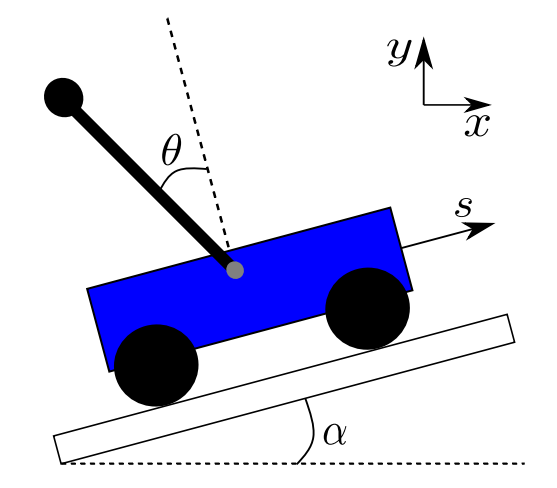
\includegraphics[scale=0.5]{fig/pendulo}
	\caption{Pêndulo Invertido}
\end{figure}
\paragraph{}Definindo ainda $v = \dot{s}$ e $\omega = \dot{\theta}$ escreve-se a dinâmica em malha aberta como,
\begin{gather}
	\begin{split}
			\begin{bmatrix}
			1 & 0 & 0 & 0 \\
			0 & 1 & 0 & 0 \\
			0 & 0 & M+m & -mlcos(\theta) \\
			0 & 0 & -mlcos(\theta) & ml^2
		\end{bmatrix}\begin{bmatrix}
			\dot{s} \\ \dot{\theta} \\ \dot{v} \\ \dot{\omega}
		\end{bmatrix} = \begin{bmatrix}
			0 & 0 & 1 & 0 \\
			0 & 0 & 0 & 1 \\
			0 & 0 & -k_v & -mlsin(\theta)\omega \\
			0 & mglcos(\alpha)sinc(\theta) & 0 & 0
		\end{bmatrix}\begin{bmatrix}
			s \\ \theta \\ v \\ \omega
		\end{bmatrix} \\
	+ \begin{bmatrix}
		0 \\ 0 \\ 1 \\ 0
	\end{bmatrix}u + \begin{bmatrix}
	0 \\ 0 \\ -(M+m)gsinc(\alpha) \\ mglcos(\theta)sinc(\alpha)
\end{bmatrix}\alpha
	\end{split}
\end{gather}
\paragraph{} Fazendo $\bar{\alpha} = sinc(\alpha)\alpha$ escreve-se o sistema descritor quasi-LPV como,
\begin{gather}
	\bm{E}(x)\dot{\bm{x}} = \bm{A}(x)\bm{x} + \bm{B_u}u + \bm{B_\alpha}(x)\bar{\alpha} \\
		\begin{split}
		\begin{bmatrix}
			1 & 0 & 0 & 0 \\
			0 & 1 & 0 & 0 \\
			0 & 0 & M+m & -mlcos(\theta) \\
			0 & 0 & -mlcos(\theta) & ml^2
		\end{bmatrix}\begin{bmatrix}
			\dot{s} \\ \dot{\theta} \\ \dot{v} \\ \dot{\omega}
		\end{bmatrix} = \begin{bmatrix}
			0 & 0 & 1 & 0 \\
			0 & 0 & 0 & 1 \\
			0 & 0 & -k_v & -mlsin(\theta)\omega \\
			0 & mglcos(\alpha)sinc(\theta) & 0 & 0
		\end{bmatrix}\begin{bmatrix}
			s \\ \theta \\ v \\ \omega
		\end{bmatrix} \\
		+ \begin{bmatrix}
			0 \\ 0 \\ 1 \\ 0
		\end{bmatrix}u + \begin{bmatrix}
			0 \\ 0 \\ -(M+m)g \\ mglcos(\theta)
		\end{bmatrix}\bar{\alpha}
	\end{split}
\end{gather}


\subsection{Representação Takagi-Sugeno Via Não Linearidade de Setor}
\paragraph{}Nessa seção será utilizada a técnica de não linearidade de setor para buscar um modelo Takagi-Sugeno exato dentro de um domínio compacto. São escolhidas as seguintes não linearidades:
\begin{gather}
	\begin{cases}
		z_1 = cos(\theta) \\
		z_2 = sin(\theta)\omega \\
		z_3 = cos(\alpha)sinc(\theta)
	\end{cases}
\end{gather}
 \paragraph{}Dessa forma obtemos um modelo dinâmico na forma,
 \begin{gather}
 %	\dot{\hat{\bm{x}}} = \bm{f(x)}\bm{x} + \bm{B_u}u + \bm{g(x)}\bar{\alpha} \\
 	 	\dot{\bm{x}} =  
 	 	\Biggl\{\begin{bmatrix}
 	 		1 & 0 & 0 & 0 \\
 	 		0 & 1 & 0 & 0 \\
 	 		0 & 0 & M+m & -mlz_1(x) \\
 	 		0 & 0 & -mlz_1(x) & ml^2
 	 	\end{bmatrix}\Biggr\}^{-1}	\Biggl\{\begin{bmatrix}
 			0 & 0 & 1 & 0 \\
 			0 & 0 & 0 & 1 \\
 			0 & 0 & -k_v & -mlz_2(x) \\
 			0 & mglz_3(x,\alpha) & 0 & 0
 		\end{bmatrix}\begin{bmatrix}
 			s \\ \theta \\ v \\ \omega
 		\end{bmatrix} 
 		+ \begin{bmatrix}
 			0 \\ 0 \\ 1 \\ 0
 		\end{bmatrix}u + \begin{bmatrix}
 			0 \\ 0 \\ -(M+m)g \\ mglz_1(x)
 		\end{bmatrix}\bar{\alpha}	\Biggl\} \\
 	\dot{\bm{x}} = \bm{f(\bm{x},\bm{u},\bm{\hat{\alpha}})}
 \end{gather}
\paragraph{} Como $\dot{\bm{x}} = \bm{f(0,0,0)} = 0$ podemos utilizar a técnica da não linearidade de setor. Tomando a condição de que estamos projetando um controlador para atuar em um terreno com inclinação máxima e minima conhecidas de forma que $\alpha \in$ [-10\textdegree ,10\textdegree], além de que da geometria do problema $\theta \in$ [-80\textdegree ,80\textdegree], e assumindo que a velocidade angular do pendulo varie como $\omega \in$ [-$\frac{pi}{9}(\frac{rad}{s})$ ,$\frac{pi}{9}(\frac{rad}{s})$].


\noindent \begin{minipage}{.25 \linewidth}
\begin{gather}
	a_{1}^{max} = \max z_1 =  1 \\
	a_{1}^{min} = \min z_1  = 0.1736 \\	
\end{gather}
\end{minipage}
\hfill
 \begin{minipage}{.25 \linewidth}
	\begin{gather}
		a_{2}^{max} = \max z_2 =  0.3438 \\
		a_{2}^{min} = \min z_2 = -0.3431 \\	
	\end{gather}
\end{minipage}
\hfill
\begin{minipage}{.25 \linewidth}
	\begin{gather}
		a_{3}^{max} =  \max z_3 = 1 \\
		a_{3}^{min} = \max z_3 = 0.6946 \\	
	\end{gather}
\end{minipage}
\paragraph{}Podemos escrever as funções de pertinência utilizando a ideia de pertencimento a uma reta ligando os extremos das não linearidades de forma que $z_i \in [a_i^{\min},a_i^{\max}]$,
\begin{gather}
		z_i(x) = \omega_{i}^{\min}(x) a_i^{\min} + \omega_{i}^{\max}(x) a_i^{\max} \\
	z_i(x) = (1 -\omega_{i}^{\max}(x) ) a_i^{\min} + \omega_{i}^{\max}(x)a_i^{\max} \\
	 \boxed{\omega_{i}^{\max}(x) = \frac{z_i(x) - a_i^{\min}}{a_i^{\max} - a_i^{\min}} , \forall{i=1,2,3}} 
\end{gather}
\paragraph{}Onde $\omega_{i}^{\min}(x) = 1 - \omega_{i}^{\max}(x)$ de forma que definimos as funções de pertencimento das não linearidades como,
\noindent \begin{minipage}{.25 \linewidth}
	\begin{gather}
	\omega_{1}^{\max}(x)  =  \frac{cos(\theta) - 1}{1-0.1736} \\
		\omega_{1}^{\min}(x) = 1 - \frac{cos(\theta) - 1}{1-0.1736} \\	
	\end{gather}
\end{minipage}
\hfill
\begin{minipage}{.25 \linewidth}
	\begin{gather}
		\omega_{2}^{max}(x) = \frac{sin(\theta)\omega + 0.3438}{0.3438 + 0.3438} \\
		\omega_{2}^{min}(x) = 1- \frac{sin(\theta)\omega + 0.3438}{0.3438 + 0.3438} \\	
	\end{gather}
\end{minipage}
\hfill
\begin{minipage}{.25 \linewidth}
	\begin{gather}
		\omega_{3}^{max}(x) = \frac{cos(\alpha)sinc(\theta) - 0.6946}{1-0.6946}  \\
		\omega_{3}^{min}(x) = 1-\frac{cos(\alpha)sinc(\theta) - 0.6946}{1-0.6946} \\	
	\end{gather}
\end{minipage}
\paragraph{}É possível notar que com 3 não linearidade teremos 8 vértice/regras ($2^{3}$) construir então a pertinência da regra como o produtório das funções de pertencimento de cada vértice,
\paragraph{Regra 1:} $z_1 = a_1^{max}, z_2 = a_2^{max}, z_3 = a_3^{max}$, $\eta_1(x) = \omega_{1}^{\max}(x)\omega_{2}^{\max}(x)\omega_{3}^{\max}(x) $
\paragraph{}Então, 
\begin{gather}
	\bm{E}_1(\bm{z})\dot{x} = \bm{A}_1(\bm{z})\bm{x} + \bm{B_u}u + \bm{B_{\alpha_{1}}}(\bm{z})\bar{\alpha}
\end{gather} 
\paragraph{Regra 2:} $z_1 = a_1^{\max}, z_2 = a_2^{\max}, z_3 = a_3^{\min}$, $\eta_2(x) = \omega_{1}^{\max}(x)\omega_{2}^{\max}(x)\omega_{3}^{\min}(x) $
\paragraph{}Então, 
\begin{gather}
	\bm{E}_2(\bm{z})\dot{x} = \bm{A}_2(\bm{z})\bm{x} + \bm{B_u}u + \bm{B_{\alpha_{2}}}(\bm{z})\bar{\alpha} \\
	\centering{\vdots}
\end{gather} 
\paragraph{Regra 8:} $z_1 = a_1^{\min}, z_2 = a_2^{\min}, z_3 = a_3^{\min}$, $\eta_8(x) = \omega_{1}^{\min}(x)\omega_{2}^{\min}(x)\omega_{3}^{\min}(x) $
\paragraph{}Então,
\begin{gather}
	\bm{E}_8(\bm{z})\dot{x} = \bm{A}_8(\bm{z})\bm{x} + \bm{B_u}u + \bm{B_{\alpha_{8}}}(\bm{z})\bar{\alpha} \\
\end{gather} 
\paragraph{}De forma que,
\begin{gather}
	\eta(x) = \sum_{i=1}^{8}\eta_i(x) = 1
\end{gather}
\paragraph{}Note que $\eta(x)$ pertence ao simplex unitário, uma vez que as funções de pertinências podem ser vistas como funções de pertinência já normalizadas. Assim podemos escrever o modelo fuzzy do sistema como,
\begin{gather}
\bm{E}(\eta(x))\dot{\bm{x}} = \bm{A}(\eta(x))\bm{x} + \bm{B_u}u + \bm{B_{\alpha}}(\eta(x))\bar{\alpha} \\
\boxed{\sum_{i=1}^{8}\eta_i(x)\bm{E}_i\dot{\bm{x}} = \sum_{i=1}^{8}\eta_i(x)\bm{A}_{i}\bm{x} + \sum_{i=1}^{8}\eta_i(x)\bm{B_u}u + \sum_{i=1}^{8}\eta_i(x)\bm{B_{\alpha_{i}}}\bar{\alpha}}
\end{gather}
\subsection{Código - ScriptTakagiSugenoModel.m}

\begin{lstlisting}[language=Matlab, caption= Script Constrói Modelo TS]
	clear
	clc
	disp('++++++++++++++++++++++++++++++++++++')
	disp('--> Running File "ScripTakagiSugenoModel.m"')
	disp('++++++++++++++++++++++++++++++++++++')
	syms M m l g kv real
	syms z1 z2 z3 real
	
	Ez = [1 0 0 0;...
	0 1 0 0;...
	0  0 M+m -m*l*z1;...
	0  0 -m*l*z1 m*l^2]; 
	
	Az = [0 0 1 0;...
	0 0 0 1;...
	0 0 -kv -m*l*z2;...
	0 m*g*l*z3 0 0];
	
	Bz = [0;0;1;0];
	
	Baz = [0;0; -(M+m)*g;m*g*l*z1];
	
	syms s theta v omega alfa sinctheta real
	
	
	
	%% Define Function sinc(x) = sin(x)/x  
	sinceq = @(x) sin(x)/x;
	%% Implementa Funcao para Pegar Pertencimento da Regra
	getw = @(gx,max,min) (gx-min)/(max - min);
	%% Sector Non Linearities 
	Z1 = subs(z1,cos(theta));
	Z2 = subs(z2,sin(theta)*omega);
	Z3 = subs(z3,cos(alfa)*sinctheta);
	Z = [Z1;Z2;Z3];
	%% Acha o Minimo de Z1
	IntervalTheta = [-deg2rad(80) deg2rad(80)];
	it =1;
	minZ1= 100;
	maxZ1 =0;
	for th = IntervalTheta(1):0.0175:IntervalTheta(2)
	teste(it) = cos(th);
	if teste(it) < minZ1
	minZ1 = teste(it);
	end
	if teste(it) > maxZ1
	maxZ1 = teste(it);
	end
	it = it+1;
	end
	

	az1max = maxZ1;
	az1min = minZ1;
	wz1max = getw(Z1,az1max,az1min);
	wz1min = 1 - wz1max;
	
	
	%% Acha o Minimo de Z2
	it =1;
	minZ2= 100;
	maxZ2 =0;
	IntervalOmega = [-deg2rad(20) deg2rad(20)];
	for th = IntervalTheta(1):0.0175:IntervalTheta(2)
	for om = IntervalOmega(1):0.0175:IntervalOmega(2)
	teste(it) = sin(th)*om;
	if teste(it) < minZ2   
	minZ2 = teste(it);
	end
	if teste(it) > maxZ2
	maxZ2 = teste(it);
	end
	it = it+1;
	end
	end
	
	
	az2max = maxZ2;
	az2min = minZ2;
	wz2max = getw(Z2,az2max,az2min);
	wz2min = 1 - wz2max; 
	
	
	%% Acha o Minimo de Z3
	it =1;
	minZ3= 100;
	maxZ3 =0;
	%   IntervalAlfa = [-0.1745 0.1745];
	IntervalAlfa = [-deg2rad(10) deg2rad(10)];
	for th = IntervalTheta(1):0.0175:IntervalTheta(2)
	for al = IntervalAlfa(1):0.0175:IntervalAlfa(2)
	teste(it) = cos(al)*sinceq(th);
	if th == 0
	teste(it) = cos(al); 
	end
	if teste(it) < minZ3
	minZ3 = teste(it);
	end
	if teste(it) > maxZ3
	maxZ3 = teste(it);
	end
	it = it+1;
	end
	end
	
	
	az3max = maxZ3;
	az3min = minZ3;
	wz3max = getw(Z3,az3max,az3min);
	wz3min = 1 - wz3max ;
	
	%% Define Vertices
	vertices = 2^(length(Z))
	E_ = cell(vertices,1);
	A_ = cell(vertices,1);
	Bu_ = cell(vertices,1);
	Ba_ = cell(vertices,1);
	%% Regra 1 max max max
	E_{1} = subs(Ez,z1,az1max);
	A_{1} = subs(Az,[z2 z3],[az2max az3max ]);
	Bu_{1} = Bz;
	Ba_{1} = subs(Baz,z1,az1max);
	h(1) = wz1max*wz2max*wz3max;
	%% Regra 2 max max min
	E_{2} = subs(Ez,z1,az1max);
	A_{2} = subs(Az,[z2 z3],[az2max az3min ]);
	Bu_{2} = Bz;
	Ba_{2} = subs(Baz,z1,az1max);
	h(2) = wz1max*wz2max*wz3min;
	%% Regra 3 max min max
	E_{3} = subs(Ez,z1,az1max);
	A_{3} = subs(Az,[z2 z3],[az2min az3max ]);
	Bu_{3} = Bz;
	Ba_{3} = subs(Baz,z1,az1max);
	h(3) = wz1max*wz2min*wz3max;
	%% Regra 4 max min min
	E_{4} = subs(Ez,z1,az1max);
	A_{4} = subs(Az,[z2 z3],[az2min az3min ]);
	Bu_{4} = Bz;
	Ba_{4} = subs(Baz,z1,az1max);   
	h(4) = wz1max*wz2min*wz3min;
	%% Regra 5 min max max
	E_{5} = subs(Ez,z1,az1min);
	A_{5} = subs(Az,[z2 z3],[az2max az3max ]);
	Bu_{5} = Bz;
	Ba_{5} = subs(Baz,z1,az1min);  
	h(5) = wz1min*wz2max*wz3max;
	%% Regra 6 min max min
	E_{6} = subs(Ez,z1,az1min);
	A_{6} = subs(Az,[z2 z3],[az2max az3min ]);
	Bu_{6} = Bz;
	Ba_{6} = subs(Baz,z1,az1min);  
	h(6) = wz1min*wz2max*wz3min;
	%% Regra 7 min min max
	E_{7} = subs(Ez,z1,az1min);
	A_{7} = subs(Az,[z2 z3],[az2min az3max ]);
	Bu_{7} = Bz;
	Ba_{7} = subs(Baz,z1,az1min); 
	h(7) = wz1min*wz2min*wz3max;
	%% Regra 8 min min min
	E_{8} = subs(Ez,z1,az1min);
	A_{8} = subs(Az,[z2 z3],[az2min az3min ]);
	Bu_{8} = Bz;
	Ba_{8} = subs(Baz,z1,az1min); 
	h(8) = wz1min*wz2min*wz3min;
	
	%% check if h belongs to unitary simplex
	test = simplify(sum(h))
	if test == 1
	disp('--> h belogs to the unitary simplex')
	else
	error('h doesnt belong to the unitary simplex')
	end
	
	
	%% Global Descriptor System
	vertices = 8;
	subvecParam = [M m l g kv];
	subvecValues = [1.5 0.3 0.3 9.78 1];
	
	for i =1:vertices
	E_{i} = double(subs(E_{i},subvecParam,subvecValues));
	A_{i} = double(subs(A_{i},subvecParam,subvecValues));
	Bu_{i} = double(subs(Bu_{i},subvecParam,subvecValues));
	Ba_{i} = double(subs(Ba_{i},subvecParam,subvecValues));
	% C_{i} = [0 0 1 0; 0 0 0 1];
	C_{i} = eye(4);
	end
	
	% Define a pertinencia da regra como variavel global
	%para ser usada pelo controlador
	global PertinenciaNormalizada
	PertinenciaNormalizada.h = h;
	
	% Define vertices do sistema usados para controle
	global DescriptorSystemDynamics
	
	DescriptorSystemDynamics.E = E_;
	DescriptorSystemDynamics.A = A_;
	DescriptorSystemDynamics.Bu = Bu_;
	DescriptorSystemDynamics.Ba = Ba_;
	DescriptorSystemDynamics.C = C_;
	
	disp('--> Takagi Sugeno Model Obtained')
	disp('+++++++++++++++++++++++++++++++++++++++++++')
\end{lstlisting}



\section{Controle}
\subsection{Lei de Controle PDC}
\paragraph{}A lei de controle PDC toma a forma,
\begin{gather}
	\boxed{u = \sum_{j=1}^{8}\eta_j(x)\bm{K_j}\bm{x}}	
\end{gather}
\paragraph{}Além disso, as seguintes afirmações do Lemma de Finsler serão utilizadas,
\begin{gather}
	\begin{cases}
		\hat{\bm{x}}'\bm{\mathcal{Q}}\hat{\bm{x}} < 0, \forall\bm{\mathfrak{B}}\hat{\bm{x}} = 0 \\
	\bm{\mathcal{Q}} + \bm{\mathcal{X}}\bm{\mathfrak{B}} + \bm{\mathfrak{B}}'\bm{\mathcal{X}} < 0	
	\end{cases}
\label{Finsler}
\end{gather}
\paragraph{}Definindo uma função de Lyapunov quadrática com os estados tal que $\bm{P}>0$, 
\begin{gather}
	\bm{V} = \bm{x}'\bm{P}\bm{x} \\
	\dot{\bm{V}} = \dot{\bm{x}}'\bm{P}\bm{x} + \bm{x}'\bm{P}\dot{\bm{x}}' < 0\\
	\dot{\bm{V}} = \begin{bmatrix}
		\bm{x}' & \dot{\bm{x}}' & \hat{\alpha}'
	\end{bmatrix}\begin{bmatrix}
	\zero & \bm{P} & \zero \\
	* & \zero & \zero \\
	* & * & \zero
\end{bmatrix}\begin{bmatrix}
\bm{x} \\ \dot{\bm{x}} \\ \hat{\alpha}
\end{bmatrix} < 0, \forall\bm{\mathfrak{B}}\hat{\bm{x}} = 0
\end{gather}
\paragraph{}Para obter $\mathfrak{B}$ vamos tomar a equação da dinâmica em malha fechada,
\begin{gather}
	\sum_{i=1}^{8}\eta_i(x)\bm{E}_i\dot{\bm{x}} = \sum_{i=1}^{8}\sum_{j=1}^{8}\eta_i(x)\eta_j(x)\big(\bm{A}_{i}+\bm{B_{u_{i}}}\bm{K}_{j}\big)\bm{x}  + \sum_{i=1}^{8}\eta_i(x)\bm{B_{\alpha_{i}}}\bar{\alpha} \\
	\bm{E}(\eta(x))\dot{\bm{x}} = \big(\bm{A}(\eta(x))+\bm{B_u}(\eta(x))\bm{K}(\eta(x))\big)\bm{x} + \bm{B_{\alpha}}(\eta(x))\bar{\alpha} \\
	\begin{bmatrix}
		\bm{A}(\eta(x))+\bm{B_u}(\eta(x))\bm{K}(\eta(x)) & -\bm{E}(\eta(x)) & \bm{B_{\alpha}}(\eta(x))
			\end{bmatrix}\begin{bmatrix}
			\bm{x} \\ \dot{\bm{x}} \\ \hat{\alpha}
		\end{bmatrix} = 0
\end{gather}
\paragraph{}De forma que $\mathfrak{B} = 	\begin{bmatrix}
	\bm{A}(\eta(x))+\bm{B_u}(\eta(x))\bm{K}(\eta(x)) & -\bm{E}(\eta(x)) & \bm{B_{\alpha}}(\eta(x))
\end{bmatrix}$ e tomando as variveis de folga, $\bm{\mathcal{X}} = \begin{bmatrix}
\bm{\mathcal{X}}_{1} \\ \bm{\mathcal{X}}_{2} \\ \bm{\mathcal{X}}_{3}
\end{bmatrix} = \begin{bmatrix}
\bm{\mathcal{X}}^{-T} \\ \mu\bm{\mathcal{X}}^{-T} \\ \zero
\end{bmatrix} $ onde $\mu$ é um escalar positivo. Tomando então a segunda relação de Finsler mostrada em \eqref{Finsler},
\begin{gather}
	\begin{split}
	\begin{bmatrix}
		\zero & \bm{P} & \zero \\
		* & \zero & \zero \\
		* & * & \zero
	\end{bmatrix} + \begin{bmatrix}
	\bm{\mathcal{X}}^{-T} \\ \mu\bm{\mathcal{X}}^{-T} \\ \zero
\end{bmatrix}	\begin{bmatrix}
\bm{A}(\eta(x))+\bm{B_u}(\eta(x))\bm{K}(\eta(x)) & -\bm{E}(\eta(x)) & \bm{B_{\alpha}}(\eta(x))
\end{bmatrix} \\
+ 	\begin{bmatrix}
	\bm{A}(\eta(x))'+\bm{K}(\eta(x))'\bm{B_u}(\eta(x))' \\ -\bm{E}(\eta(x))' \\ \bm{B_{\alpha}}(\eta(x))'
\end{bmatrix} \begin{bmatrix}
\bm{\mathcal{X}}^{-1} & \mu\bm{\mathcal{X}}^{-1} & \zero
\end{bmatrix} < 0
\end{split} \\
\hspace{-1cm}\tiny{\begin{bmatrix}
	\bm{\mathcal{X}}^{-T}\Biggl\{\Af + \Buf\Kf\Biggr\} + \Biggl\{\Af' + \Kf'\Buf'\Biggr\}\bm{\mathcal{X}}^{-1} & \bm{P} - \bm{\mathcal{X}}^{-T}\Ef + \mu\Biggl\{\Af' + \Kf'\Buf'\Biggr\}\bm{\mathcal{X}}^{-1}  & \bm{\mathcal{X}}^{-T}\Baf \\
	* & -\mu\bm{\mathcal{X}}^{-T}\Ef - \mu\Ef'\bm{\mathcal{X}}^{-1} & \mu\bm{\mathcal{X}}^{-T}\Baf \\
	* & * & \zero
\end{bmatrix} < 0}
\end{gather}
\paragraph{}Fazendo uma transformação de congruência multiplicando pelo lado direito por $\begin{bmatrix}
	\bm{\mathcal{X}} & \zero & \zero \\
	* & \bm{\mathcal{X}} & \zero \\
	* & * & \zero
\end{bmatrix}$ e por sua transposta no lado esquerdo,
\begin{gather}
	\hspace{-1.85cm}\small{\begin{bmatrix}
		\Af\bm{\mathcal{X}} + \Buf\Kf\bm{\mathcal{X}} + \bm{\mathcal{X}}'\Af' + \bm{\mathcal{X}}'\Kf\Buf' & \bm{\mathcal{X}}'\bm{P}\bm{\mathcal{X}} - \Ef\bm{\mathcal{X}} + \mu\bm{\mathcal{X}}'\Af' + \mu\bm{\mathcal{X}}'\Kf'\Buf' & \zero \\
		* & -\mu\Ef\bm{\mathcal{X}}-\mu\bm{\mathcal{X}}'\Ef' & \zero \\
		* & * & \zero
	\end{bmatrix} < 0}
\end{gather}
\paragraph{}Fazendo uma transformação do tipo $\bar{\bm{P}} = \bm{\mathcal{X}}'\bm{P}\bm{\mathcal{X}}$ e $\bm{\mathcal{Y}}(\eta(x)) = \Kf\bm{\mathcal{X}}$ e eliminando as colunas com zeros para ajudar na implementação, obtemos a seguinte desigualdade matricial.
\begin{gather}
\hspace{-1.5cm}	\begin{bmatrix}
		\Af\bm{\mathcal{X}} + \bm{\mathcal{X}}'\Af' + \color{red}{\Buf\bm{\mathcal{Y}}(\eta(x))} + \bm{\mathcal{Y}}(\eta(x))'\Buf' & \bar{\bm{P}} - \Ef\bm{\mathcal{X}} + \mu\big(\bm{\mathcal{X}}'\Af' + \color{red}{\bm{\mathcal{Y}}(\eta(x))'\Buf'}\color{black}\big) \\
		* & -\mu\big(\Ef\bm{\mathcal{X}}+\bm{\mathcal{X}}'\Ef'\big)
	\end{bmatrix} < 0
\end{gather}
\paragraph{}Chamando essa desigualdade matricial acima de $\bm{\Phi}$, homogenizando os termos, e lembrando que $(.)(\eta(x)) = \sum_{i=1}^{8}\eta_{i}(.)_i$ podemos achar as condições de LMI suficientes dadas abaixo,
\begin{gather}
	\begin{cases}
		\bar{\bm{P}} > 0 \\
		\bm{\Phi}_{ii} < 0, \forall{i} \\
		\bm{\Phi}_{ij} + \bm{\Phi}_{ji} < 0, \text{onde $1 \leq i  \leq 7$ e $2 \leq j  \leq 8$} 
	\end{cases}
\end{gather}
\subsubsection{Resultados PDC Control}
\paragraph{}Uma busca foi feita para se obter o escalar $\mu$ o variando de 10 até 20 com o passo fixo de 1, e analisando os resultados dos ganhos para avaliar a escolha do escalar. Os resultados de como $\mu$ influência nos ganhos do controlador são mostrados abaixo.
\begin{figure}
	\centering
	\begin{subfigure}[b]{0.3\textwidth}
		\centering
		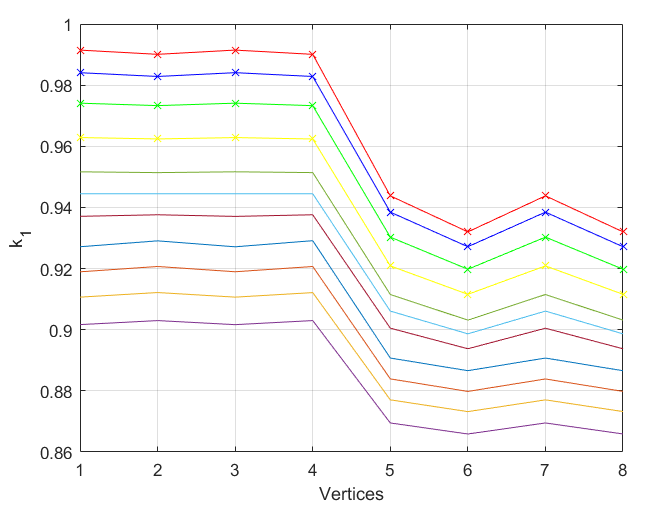
\includegraphics[scale=0.7]{fig/pdcmuk1}
		\caption{$k_1$}
	\end{subfigure}
	\hfill
	\begin{subfigure}[b]{0.45\textwidth}
		\centering
		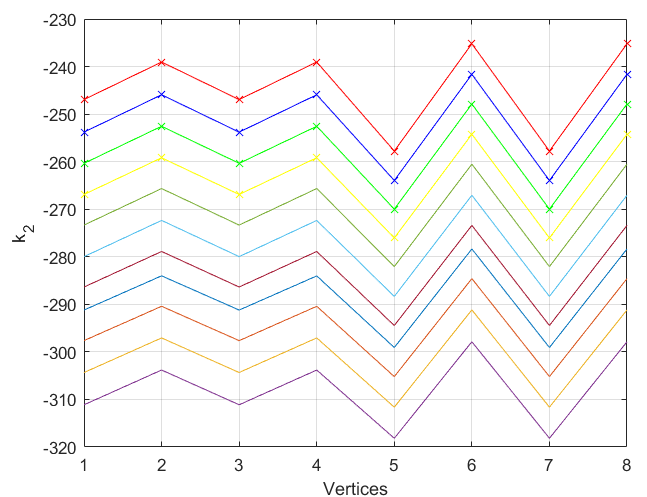
\includegraphics[scale=0.7]{fig/pdcmuk2}
		\caption{$k_2$}
	\end{subfigure}
\end{figure}
\begin{figure}
	\centering
	\begin{subfigure}[b]{0.3\textwidth}
		\centering
		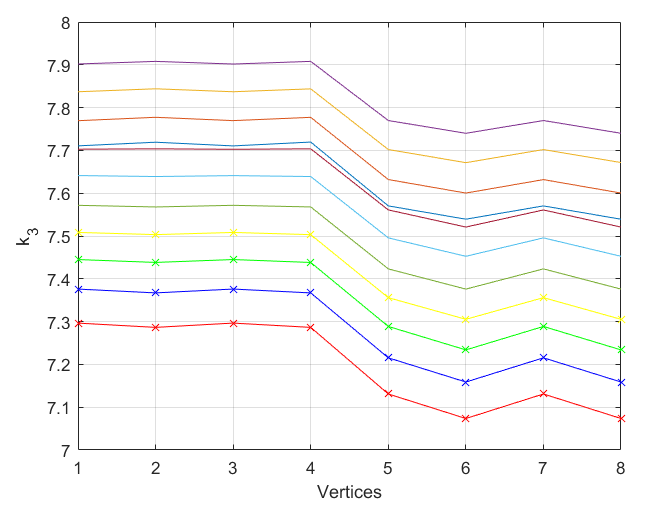
\includegraphics[scale=0.7]{fig/pdcmuk3}
		\caption{$k_3$}
	\end{subfigure}
	\hfill
	\begin{subfigure}[b]{0.45\textwidth}
		\centering
		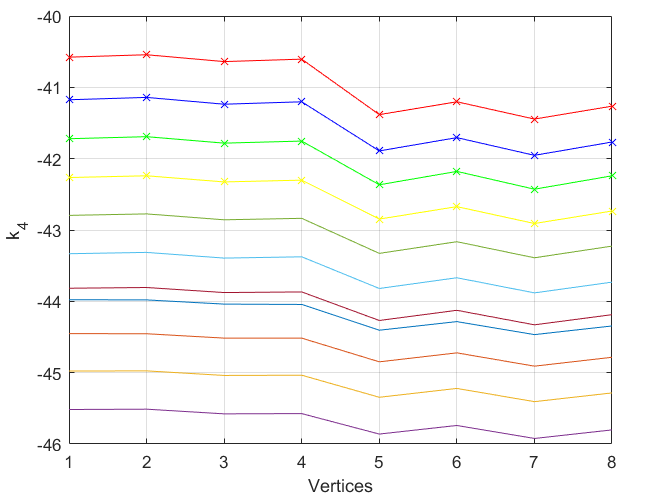
\includegraphics[scale=0.7]{fig/pdcmuk4}
		\caption{$k_4$}
	\end{subfigure}
\end{figure}
\paragraph{}Selecionando-se então $\mu=10$ os resultados factíveis da otimização do solver SeDuMi são mostrados abaixo.
\begin{lstlisting}[language=Matlab]
+++++++++++++++++++++++++++++++++++++++++++++++++++++++++++++++++
|    ID|          Constraint|   Primal residual|   Dual residual|
+++++++++++++++++++++++++++++++++++++++++++++++++++++++++++++++++
|    #1|   Matrix inequality|        6.5607e-05|      2.2051e-14|
|    #2|   Matrix inequality|        5.3298e-06|      8.1486e-14|
|    #3|   Matrix inequality|        6.5607e-05|      2.2051e-14|
|    #4|   Matrix inequality|        1.7589e-06|      8.1058e-14|
|    #5|   Matrix inequality|        6.5607e-05|      2.2051e-14|
|    #6|   Matrix inequality|        5.3298e-06|      8.1483e-14|
|    #7|   Matrix inequality|        6.5607e-05|      2.2051e-14|
|    #8|   Matrix inequality|        1.7589e-06|      8.1058e-14|
|    #9|   Matrix inequality|        6.5607e-05|      2.2051e-14|
|   #10|   Matrix inequality|        2.2195e-06|      7.5549e-14|
|   #11|   Matrix inequality|        6.5607e-05|      2.2051e-14|
|   #12|   Matrix inequality|        1.8181e-06|      8.0837e-14|
|   #13|   Matrix inequality|        6.5607e-05|      2.2051e-14|
|   #14|   Matrix inequality|        2.2196e-06|      7.5547e-14|
|   #15|   Matrix inequality|        6.5607e-05|      2.2051e-14|
|   #16|   Matrix inequality|        1.8181e-06|      8.0835e-14|
|   #17|   Matrix inequality|         8.908e-06|      4.2021e-14|
|   #18|   Matrix inequality|         1.066e-05|      4.4286e-14|
|   #19|   Matrix inequality|         8.908e-06|      4.2021e-14|
|   #20|   Matrix inequality|        1.5769e-05|      3.9693e-14|
|   #21|   Matrix inequality|        1.4005e-05|      4.0319e-14|
|   #22|   Matrix inequality|        1.5769e-05|      3.9693e-14|
|   #23|   Matrix inequality|        1.4005e-05|      4.0319e-14|
|   #24|   Matrix inequality|         8.908e-06|       4.202e-14|
|   #25|   Matrix inequality|        3.5179e-06|       3.981e-14|
|   #26|   Matrix inequality|        1.4395e-05|       3.982e-14|
|   #27|   Matrix inequality|        9.2935e-06|      4.0339e-14|
|   #28|   Matrix inequality|        1.4395e-05|       3.982e-14|
|   #29|   Matrix inequality|        9.2935e-06|      4.0339e-14|
|   #30|   Matrix inequality|         8.908e-06|       4.202e-14|
|   #31|   Matrix inequality|        1.5769e-05|      3.9692e-14|
|   #32|   Matrix inequality|        1.4005e-05|      4.0319e-14|
|   #33|   Matrix inequality|        1.5769e-05|      3.9692e-14|
|   #34|   Matrix inequality|        1.4005e-05|      4.0318e-14|
|   #35|   Matrix inequality|        1.4395e-05|       3.982e-14|
|   #36|   Matrix inequality|        9.2935e-06|      4.0339e-14|
|   #37|   Matrix inequality|        1.4395e-05|       3.982e-14|
|   #38|   Matrix inequality|        9.2935e-06|      4.0339e-14|
|   #39|   Matrix inequality|        1.3658e-05|      3.9955e-14|
|   #40|   Matrix inequality|        4.4391e-06|      3.7045e-14|
|   #41|   Matrix inequality|        1.3658e-05|      3.9955e-14|
|   #42|   Matrix inequality|        1.3658e-05|      3.9955e-14|
|   #43|   Matrix inequality|        3.6363e-06|      3.8506e-14|
|   #44|   Matrix inequality|        1.3658e-05|      3.9954e-14|
+++++++++++++++++++++++++++++++++++++++++++++++++++++++++++++++++
| A primal-dual optimal solution would show non-negative residuals.|
| In practice, many solvers converge to slightly infeasible     |
| solutions, which may cause some residuals to be negative.     |
| It is up to the user to judge the importance and impact of    |
| slightly negative residuals (i.e. infeasibilities)            |
| https://yalmip.github.io/command/check/                       |
| https://yalmip.github.io/faq/solutionviolated/                |
+++++++++++++++++++++++++++++++++++++++++++++++++++++++++++++++++
\end{lstlisting}
\paragraph{}Para simular o comportamento do sistema um Simulink foi criado como mostrado na figura.

\begin{figure}[H]
	\centering
	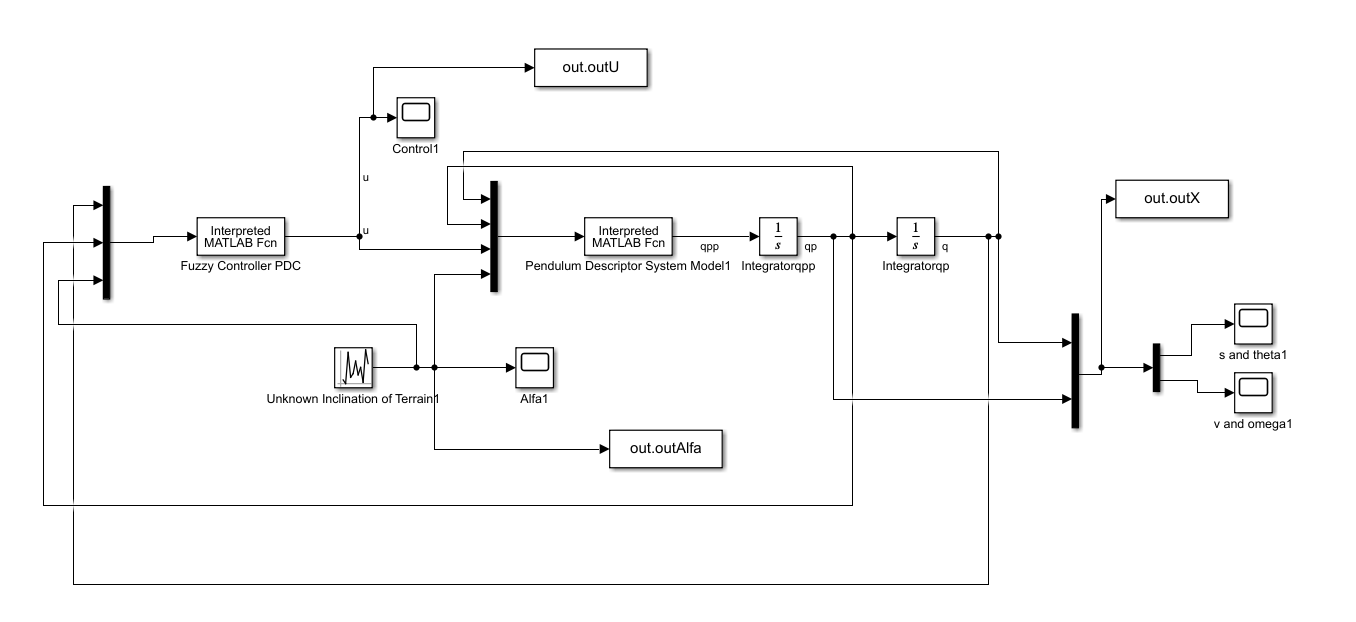
\includegraphics[scale = 0.6]{fig/PDCsimulink}
\end{figure}
\paragraph{OBS:}apesar de no simulink constar o nome "Pendulum Descriptor System Model1" o modelo implementado foi o dado por \eqref{eqdyn}.
\paragraph{}Uma simulação com 60 segundos de duração foi feita, tendo como condições iniciais $\bm{q}(0) = \begin{bmatrix}
	0 \\ \frac{\pi}{4}
\end{bmatrix}$ e $\dot{\bm{q}}(0) = \begin{bmatrix}
0 \\ 0
\end{bmatrix}$, e com a inclinação do terreno aleatória variando entre mais ou menos dez graus. Os resultados dos estados e entrada de controle são mostrados abaixo.

\begin{figure}[H]
	\centering
	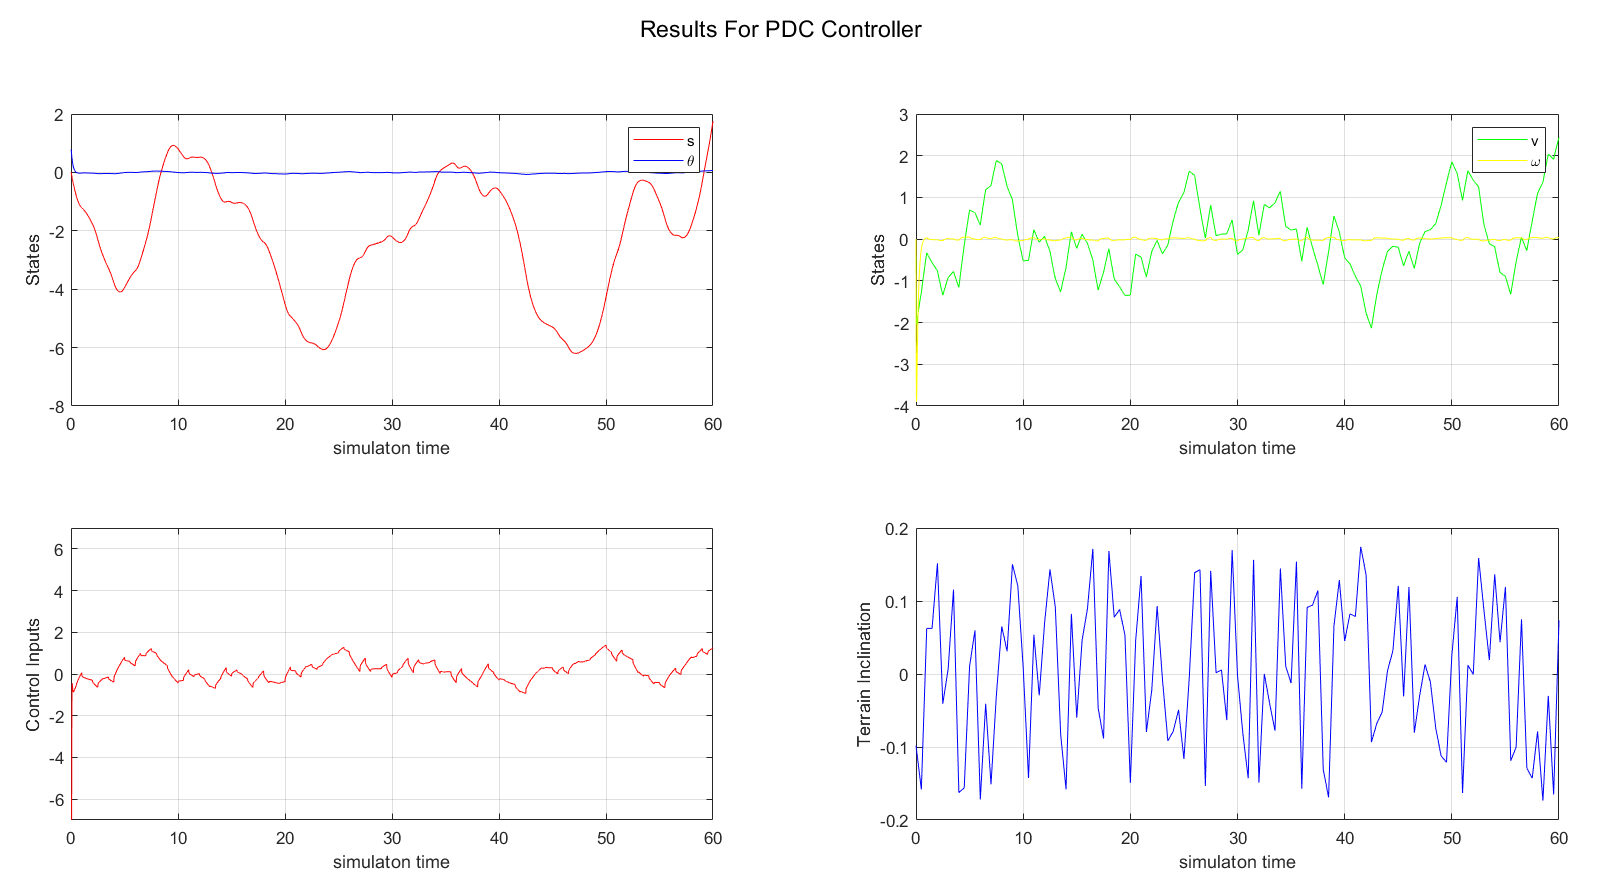
\includegraphics[scale = 0.5]{fig/PDCresult}
\end{figure}


\newpage
\subsection{Lei de Controle PDC com $\mathcal{H}_\infty$}
\paragraph{}A mesma lei de controle PDC será utilizada bem como as afirmações do Lemma de Finsler ,
\begin{gather}
	\boxed{u = \sum_{j=1}^{8}\eta_j(x)\bm{K_j}\bm{x}}	
\end{gather}
\paragraph{}Essa será uma demonstração muito mais rápida e com menos detalhes. Tomando a derivada temporal da função de Lyapunov a mesma assumirá a seguinte forma para o problema do $\mathcal{H}_\infty$. Assumindo $\bm{z} = \bm{C}\bm{x} + \bm{D_{\alpha}}\hat{\alpha}$
\begin{gather}
\dot{\bm{V}} +\frac{1}{\gamma}\bm{x}'\bm{C}'\bm{C}\bm{x} - \gamma\bar{\alpha}'\bar{\alpha} < 0\\
 \begin{bmatrix}
	\bm{x}' & \dot{\bm{x}}' & \hat{\alpha}'
\end{bmatrix}\Bigg(\begin{bmatrix}
	\zero & \bm{P} & \zero \\
	* & \zero & \zero \\
	* & * & -\gamma\bm{I}
\end{bmatrix} + \frac{1}{\gamma}\begin{bmatrix}
\bm{C}' \\ \zero \\ \bm{D_{\alpha}}'
\end{bmatrix}\begin{bmatrix}
\bm{C} & \zero & \bm{D_{\alpha}}
\end{bmatrix}\Bigg)\begin{bmatrix}
	\bm{x} \\ \dot{\bm{x}} \\ \hat{\alpha}
\end{bmatrix} < 0
\end{gather}
\paragraph{}Tomando os mesmo passos de se multiplicar pelo lado direito e esquerdo pela mesma transformação de congruência utilizada para o controlador PDC, utilizando as mesmas transformações linearizantes, utilizando complemento de Schur e eliminando as colunas de zeros para facilitar a resolução do solver SeDuMi obtemos a seguinte desigualdade matricial,
\small{\begin{gather}
	\hspace{-1cm}\begin{bmatrix}
		\Af\X + \X'\Af' + \Buf\Y + \Y'\Buf & \bar{\bm{P}} - \Ef\X + \mu(\X'\Af' + \Y'\Buf') & \X'\bm{C}' \\
		* & -\mu(\Ef\X + \X'\Ef') & \zero \\
		* & * & -\gamma\bm{I}
	\end{bmatrix}  < 0
\end{gather}}
\paragraph{}Chamando a desigualdade de $\Psi$, homogenizando os termos e lembrando que $\bar{\bm{P}} = \bm{\mathcal{X}}'\bm{P}\bm{\mathcal{X}}$ e $\bm{\mathcal{Y}}(\eta(x)) = \Kf\bm{\mathcal{X}}$, as seguintes LMIs devem ser implementadas.

\begin{gather}
	\begin{cases}
		\bar{\bm{P}} > 0 \\
		\bm{\Psi}_{ii} < 0, \forall{i} \\
		\bm{\Psi}_{ij} + \bm{\Psi}_{ji} < 0, \text{onde $1 \leq i  \leq 7$ e $2 \leq j  \leq 8$} 
	\end{cases}
\end{gather}
\subsubsection{Resultados PDC com $\mathcal{H}_{\infty}$}
\paragraph{}Uma busca foi feita para se obter o escalar $\mu$ o variando de 10 até 20 com o passo fixo de 1, e analisando os resultados dos ganhos para avaliar a escolha do escalar. Os resultados de como $\mu$ influência nos ganhos do controlador são mostrados abaixo.
\begin{figure}[H]
	\centering
	\begin{subfigure}[b]{0.3\textwidth}
		\centering
		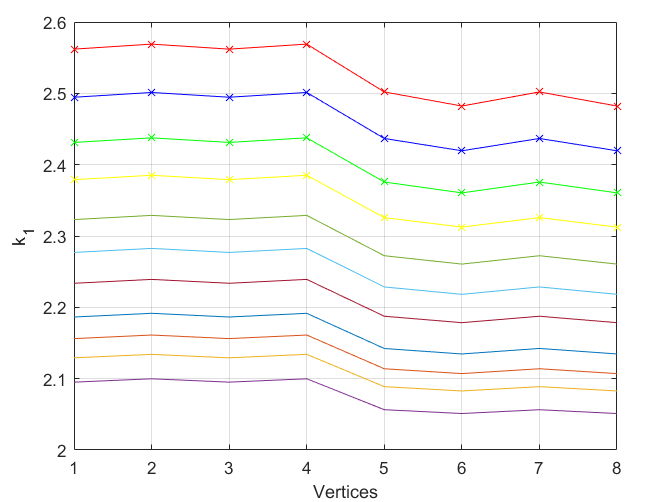
\includegraphics[scale=0.7]{fig/pdchmuk1}
		\caption{$k_1$}
	\end{subfigure}
	\hfill
	\begin{subfigure}[b]{0.45\textwidth}
		\centering
		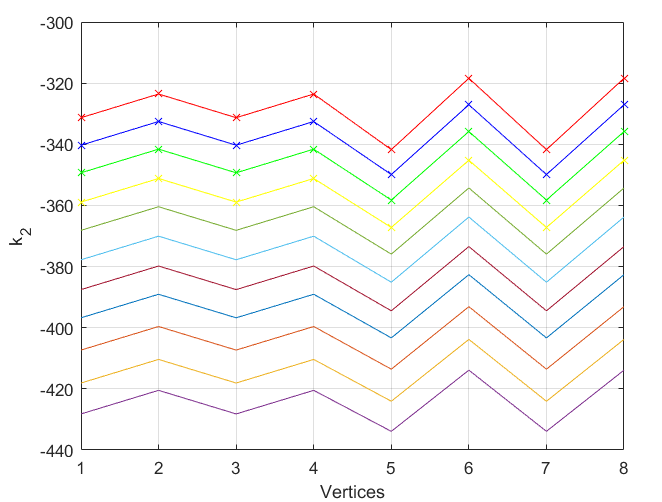
\includegraphics[scale=0.7]{fig/pdchmuk2}
		\caption{$k_2$}
	\end{subfigure}
\end{figure}
\begin{figure}[H]
	\centering
	\begin{subfigure}[b]{0.3\textwidth}
		\centering
		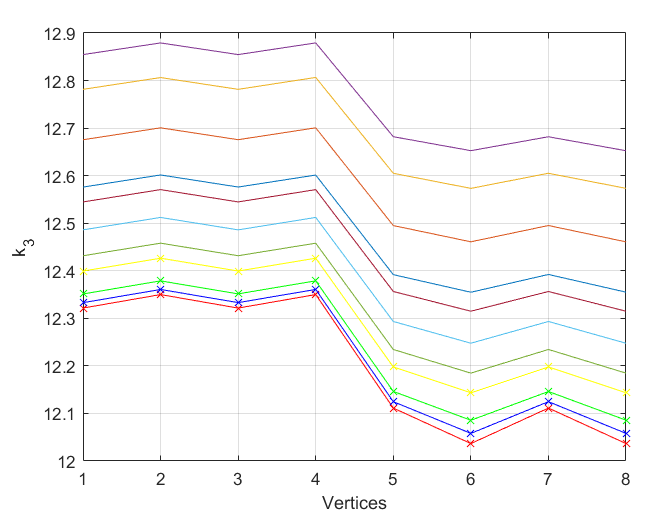
\includegraphics[scale=0.7]{fig/pdchmuk3}
		\caption{$k_3$}
	\end{subfigure}
	\hfill
	\begin{subfigure}[b]{0.45\textwidth}
		\centering
		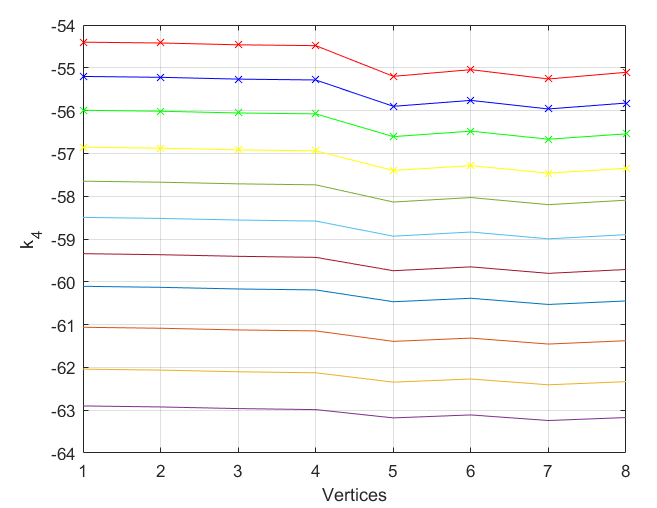
\includegraphics[scale=0.7]{fig/pdchmuk4}
		\caption{$k_4$}
	\end{subfigure}
\end{figure}
\paragraph{}Selecionando-se então $\mu=10$ os resultados factíveis da otimização do solver SeDuMi são mostrados abaixo.
\begin{lstlisting}[language=Matlab]
	+++++++++++++++++++++++++++++++++++++++++++++++++++++++++++++++++
	|    ID|          Constraint|   Primal residual|   Dual residual|
	+++++++++++++++++++++++++++++++++++++++++++++++++++++++++++++++++
	|    #1|   Matrix inequality|        2.9312e-07|       1.245e-14|
	|    #2|   Matrix inequality|        1.9837e-08|      5.6459e-14|
	|    #3|   Matrix inequality|        2.9312e-07|       1.245e-14|
	|    #4|   Matrix inequality|        3.5097e-09|      5.6862e-14|
	|    #5|   Matrix inequality|        2.9312e-07|       1.245e-14|
	|    #6|   Matrix inequality|        1.9837e-08|      5.6463e-14|
	|    #7|   Matrix inequality|        2.9312e-07|       1.245e-14|
	|    #8|   Matrix inequality|        3.5097e-09|      5.6862e-14|
	|    #9|   Matrix inequality|        2.9312e-07|       1.245e-14|
	|   #10|   Matrix inequality|        4.9461e-09|      5.3139e-14|
	|   #11|   Matrix inequality|        2.9312e-07|       1.245e-14|
	|   #12|   Matrix inequality|        3.6778e-09|       5.743e-14|
	|   #13|   Matrix inequality|        2.9312e-07|       1.245e-14|
	|   #14|   Matrix inequality|        4.9461e-09|       5.314e-14|
	|   #15|   Matrix inequality|        2.9312e-07|       1.245e-14|
	|   #16|   Matrix inequality|        3.6778e-09|      5.7426e-14|
	|   #17|   Matrix inequality|        3.1635e-08|      2.8329e-14|
	|   #18|   Matrix inequality|        3.9673e-08|      2.9228e-14|
	|   #19|   Matrix inequality|        3.1635e-08|      2.8329e-14|
	|   #20|   Matrix inequality|         5.002e-08|      2.7924e-14|
	|   #21|   Matrix inequality|         4.421e-08|      2.8477e-14|
	|   #22|   Matrix inequality|         5.002e-08|      2.7925e-14|
	|   #23|   Matrix inequality|         4.421e-08|      2.8477e-14|
	|   #24|   Matrix inequality|        3.1635e-08|      2.8329e-14|
	|   #25|   Matrix inequality|        7.0194e-09|      2.5329e-14|
	|   #26|   Matrix inequality|        4.6352e-08|      2.7937e-14|
	|   #27|   Matrix inequality|        2.7814e-08|      2.8446e-14|
	|   #28|   Matrix inequality|        4.6352e-08|      2.7937e-14|
	|   #29|   Matrix inequality|        2.7814e-08|      2.8446e-14|
	|   #30|   Matrix inequality|        3.1635e-08|      2.8329e-14|
	|   #31|   Matrix inequality|         5.002e-08|      2.7925e-14|
	|   #32|   Matrix inequality|         4.421e-08|      2.8478e-14|
	|   #33|   Matrix inequality|         5.002e-08|      2.7926e-14|
	|   #34|   Matrix inequality|         4.421e-08|      2.8477e-14|
	|   #35|   Matrix inequality|        4.6352e-08|      2.7936e-14|
	|   #36|   Matrix inequality|        2.7813e-08|      2.8446e-14|
	|   #37|   Matrix inequality|        4.6352e-08|      2.7937e-14|
	|   #38|   Matrix inequality|        2.7814e-08|      2.8446e-14|
	|   #39|   Matrix inequality|        5.1287e-08|      2.7741e-14|
	|   #40|   Matrix inequality|        9.8922e-09|      2.9111e-14|
	|   #41|   Matrix inequality|        5.1287e-08|      2.7739e-14|
	|   #42|   Matrix inequality|        5.1287e-08|      2.7741e-14|
	|   #43|   Matrix inequality|        7.3556e-09|      2.5582e-14|
	|   #44|   Matrix inequality|        5.1287e-08|      2.7739e-14|
	+++++++++++++++++++++++++++++++++++++++++++++++++++++++++++++++++
	| A primal-dual optimal solution would show non-negative residuals.|
	| In practice, many solvers converge to slightly infeasible     |
	| solutions, which may cause some residuals to be negative.     |
	| It is up to the user to judge the importance and impact of    |
	| slightly negative residuals (i.e. infeasibilities)            |
	| https://yalmip.github.io/command/check/                       |
	| https://yalmip.github.io/faq/solutionviolated/                |
	+++++++++++++++++++++++++++++++++++++++++++++++++++++++++++++++++
\end{lstlisting}
\paragraph{}Para simular o comportamento do sistema um Simulink foi criado como mostrado na figura.

\begin{figure}[H]
	\centering
	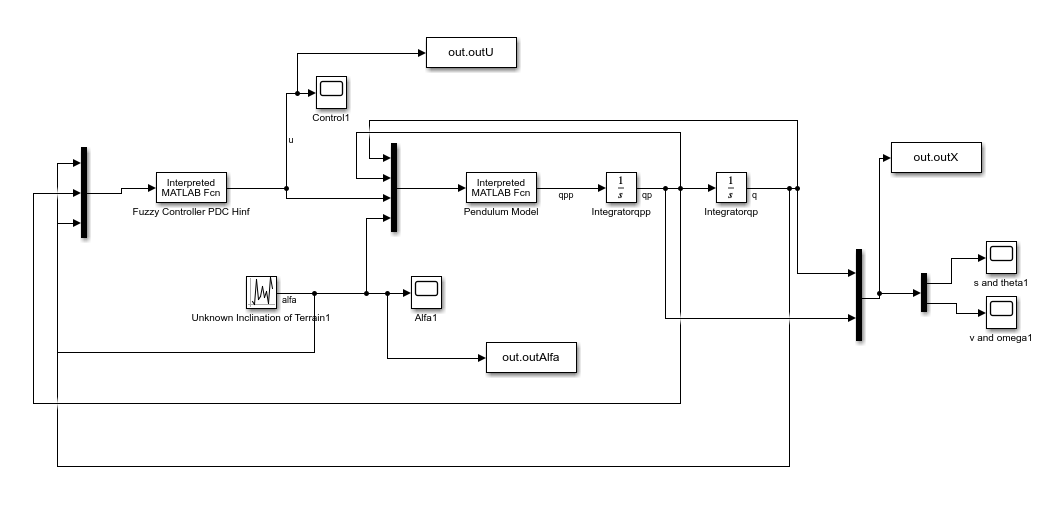
\includegraphics[scale = 0.6]{fig/PDCHsimulink}
\end{figure}
\paragraph{}Uma simulação com 60 segundos de duração foi feita, tendo como condições iniciais $\bm{q}(0) = \begin{bmatrix}
	0 \\ \frac{\pi}{4}
\end{bmatrix}$ e $\dot{\bm{q}}(0) = \begin{bmatrix}
	0 \\ 0
\end{bmatrix}$, e com a inclinação do terreno aleatória variando entre mais ou menos dez graus. Os resultados dos estados e entrada de controle são mostrados abaixo.

\begin{figure}[H]
	\centering
	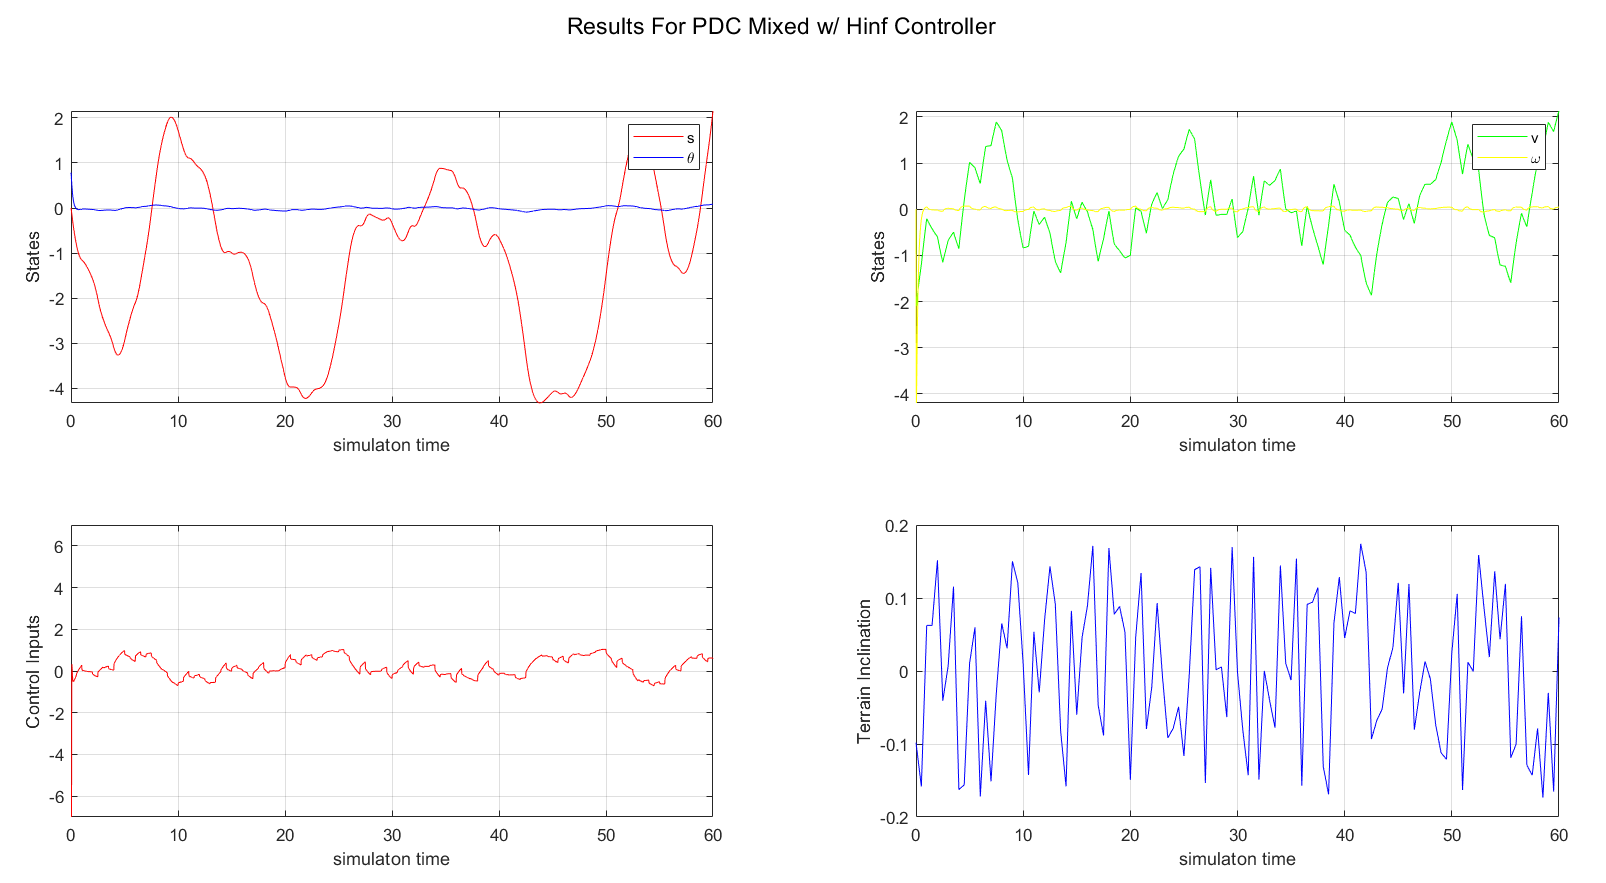
\includegraphics[scale = 0.5]{fig/PDCHresult}
\end{figure}

\section{Comparação}
\subsection{Comparando os Controladores}
\paragraph{}Para comparar ambos os controladores primeiro modificou-se o simulink para ambos estarem submetidos a uma mesma pertubação, além disso as condições iniciais também foram iguais para ambos os sistemas, e os passo do solver de integração numérica foi definido como 0.001 para ambos os controladores. Os resultados são vistos abaixo.
\begin{figure}[H]
	\centering
	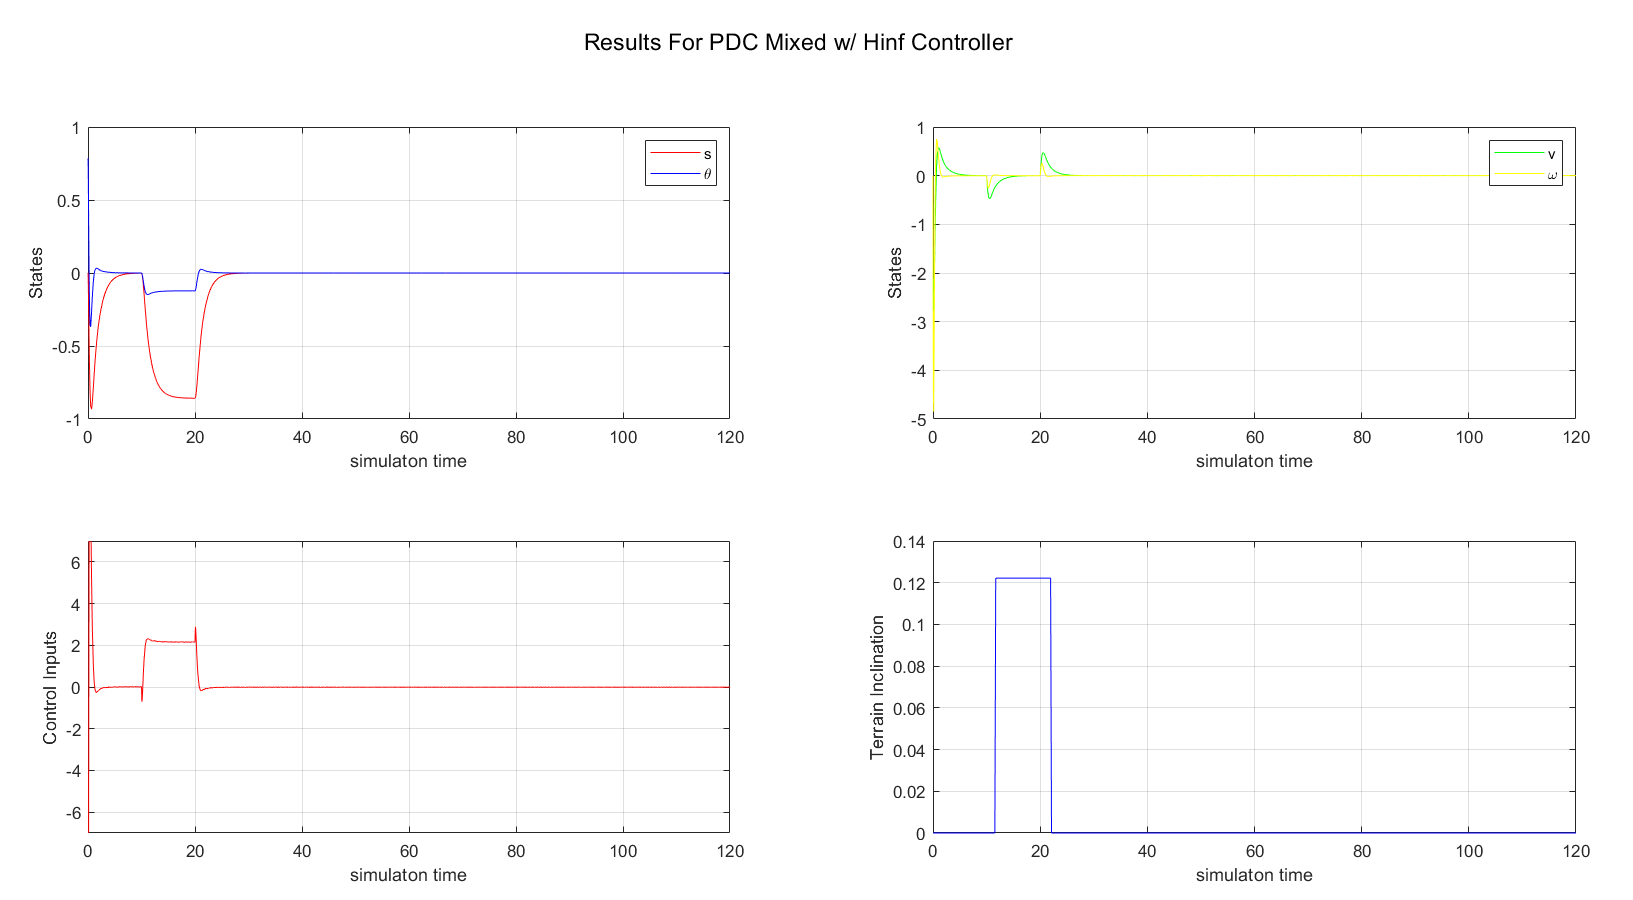
\includegraphics[scale = 0.5]{fig/PDCHinfcompare}
\end{figure}

\paragraph{}Como se esperava o controlador com $\mathcal{H}_{\infty}$ apresenta o melhor comportamento convergindo para zero no menor tempo e com menos \textit{overshoot}.
\paragraph{}As simulações podem ser testadas acessando meu repositório no github: \url{https://github.com/Jonatan29/ParallelDistributedControl/tree/master}
\end{document}
